\section{EXPERIMENTS}
\label{sec:evaluation}
%Why we need evaluation\label{sec:relevance}
The main contribution of this paper is to introduce a new approach to explanations(Hierarchical Intervention). We evaluate this new approach in a number of different ways. We perform qualitative evaluation and speed/scalability evaluation.

\begin{figure}[h]
	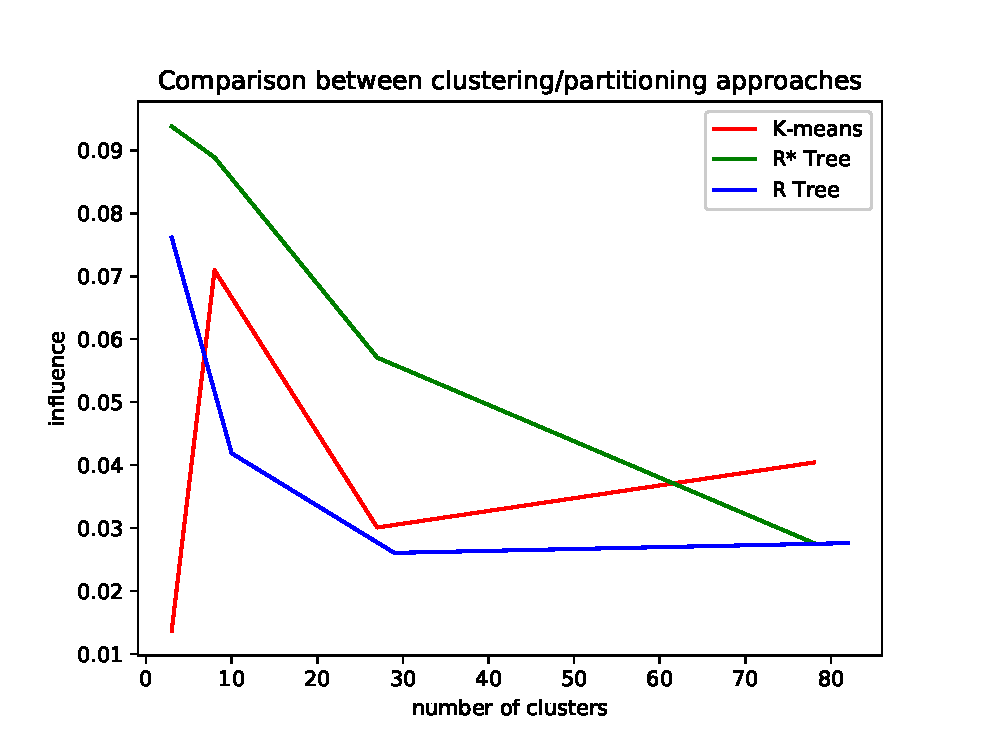
\includegraphics[width=0.96\columnwidth]{images/clustering_comparison}
	\caption{Comparison of Influence against number of clusters for K-Means, R-Tree and R*-Tree}
	\label{fig:clustering_comparison}
\end{figure}

In order to compare the different clustering techniques that we use in hierarchical intervention, we did a couple of experiments. Our solution relies on the fact that the higher the influence or intensity is a measure of the value of our explanations. We used a number of observations on the NYC TLC data to see how each clustering technique fares against the others.

\textbf{Experimental Setup}. 
In our evaluation, we will use both single-machine and multiple-machines environments. 
In the single-machine environment, we use one machine with an i7 6400 3.5 GHz CPU and 8GB of RAM. 
In a multiple-machines environment, we take Google Compute Engine as our cluster. 
The cluster has 4 nodes and all the nodes in our cluster had the same specifications.
Each machine has 1 vCPU and 3.5GB RAM.
We run Apache Spark on YARN while the Salient Features were generated with the Data Polygamy Framework running on YARN. 

{\bf Dataset}. 
In our experiment, we use the yellow and green taxi trip records as our dataset. 
This dataset includes the pick-up and drop-off location of the taxi trips and the properties for each trip, such as fare, payment method, etc,. The dataset is organized in a monthly way that each file in the dataset stores the trips within one month.
%The dataset used for this experiment was the NYC TLC data for January 2016. This data contains ~10 million trips.
Another dataset that we use for evaluation is from the Indiana Public Health Emergency Surveillance System. This data contains information about Patients in Indiana and their health issues over time and location. 

%\textbf{Experimental Setup}. We performed the evaluation on the first 5 months of data from the NYC yellow cab dataset from 2016. The data spanned ~ 50 million trips. The $k$ for our evaluation was $5$. This value was chosen after a series of experiments. We wanted the size of each partition to be large enough to support our generalization assumption. If the solution space for evaluation is small, it leads to inconsistent results. Each month represented a partition for k-folds evaluation. According to our analysis, we found that the approach works very well with low values of alpha. Fig.~\ref{fig:kfolds} shows some of the results of our evaluation for a number of observations. The lower the value of the relative distance, the better the results.

%\textbf{Experimental Setup}. The speed of each approach is simply the time taken to calculate the explanations. Since all the approaches are implemented on top of distributed systems, the time varies depending on the number of nodes used. We experimented with calculating explanations for 1,3, and 5 months in a distributed environment. For the cluster, we used Google Compute Engine nodes(1 vCPU, 3.5GB RAM, 4 nodes). All the nodes in our cluster had the same specifications. The Aggravation, Intervention and Hierarchical Intervention were tested on Apache Spark running on YARN while the Salient Features were generated with the Data Polygamy Framework running on YARN.

\subsection{Spatial partitioning methods}
\label{sec:spatial_partitioning_methods}
\begin{figure}[t]
	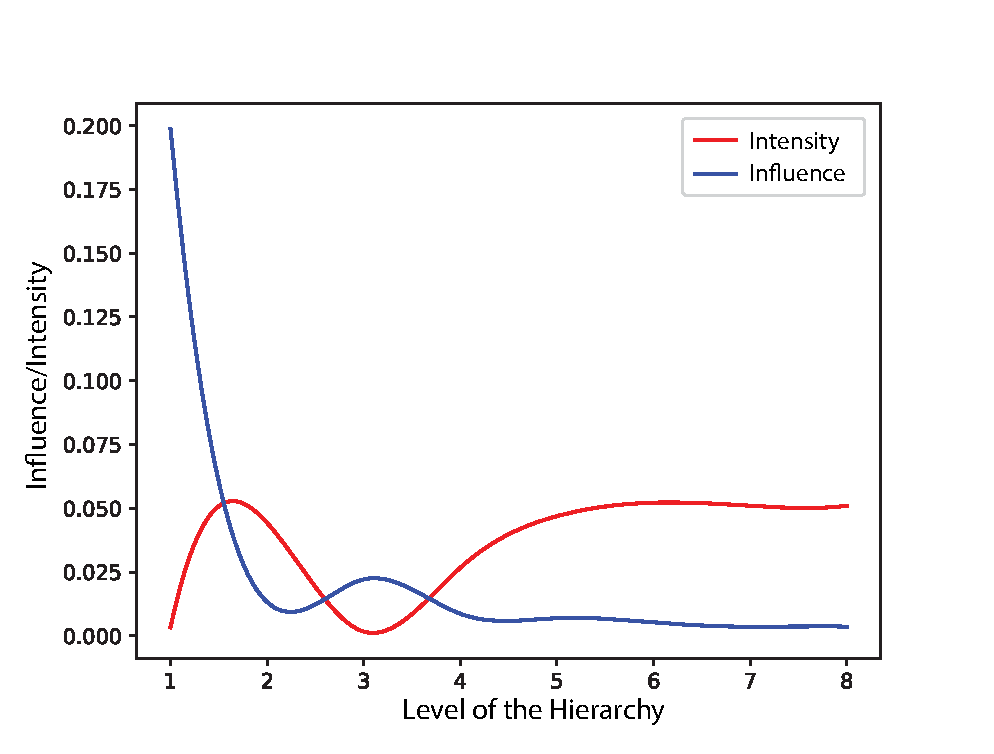
\includegraphics[width=\columnwidth]{images/hieint_passenger_count}
	\caption{Comparison of Influence and Intensity against level of hierarchy with average passenger count as observation}
	\label{fig:hieint_passenger_count}
\end{figure}
Spatial explanation requires to create spatial predicate which partition the whole dataset into different spatial partitions. In our evaluation, we consider three spatial partitioning methods, R-Tree, R* Tree and K-means. 
Fig. \ref{fig:clustering_comparison} shows the influence of different partitioning methods with a different number of clusters. 
The stability of the clustering technique is referring to its monotonicity of the explanation as a function of the number of clusters. 
It shows that R-Tree and R* Tree partitioning methods are more stable than K-Means. 
Furthermore, R* Tree has a higher influence on average compared to other approaches making it a lot more suitable for explanations.

The candidate spatial {\explanation}s are in different levels of the hierarchy. 
Fig.~\ref{fig:hieint_passenger_count} shows the {\influence} against the number of hierarchy levels where the observation is the average passenger count. 
The influence and intensity tend to oscillate when the level of hierarchy changes.
The changing shape is closer to a sinusoidal curve than an exponential or logarithmic curve. 
The reason for the oscillation is when merged to a higher level, the {\explanation} can be enhanced or weakened. 
If the children {\explanation} all have the positive intensity and influence, the parent {\explanation} will be enhanced. 
Otherwise, the value will decrease. 
%Fig.~\ref{fig:clustering_comparison} shows another observation and a plot of the influence of R-Tree and R*-Tree as well. The influence as a function of the number of clusters is a lot more monotonic here. 
%Furthermore, R* Tree has a higher influence on average compared to other approaches making it a lot more suitable for explanations.
%Reasons for selecting evaluation criteria
%The qualitative evaluation that we define is based on K-Folds cross-validation. The reason for selecting these evaluations is to measure how the top explanations provided by each approach fair as stand-alone parts of data as well as their effects on the entire dataset as a whole. Other than qualitative analysis we look at the speed and scalability of each approach for performance evaluation.



%How does each approach compare
\subsection{Influence Comparison.}
Fig.~\ref{fig:influence_comparison} shows the comparison between the influence of different approaches. Salient features and {\aggravation} have a very low influence (close to 0) compared to Intervention and hierarchical intervention. This is because the explanations provided by those approaches cover a very small portion of the entire dataset. This makes removing the associated data have a negligible impact on the entire data.
\begin{figure}[h]
	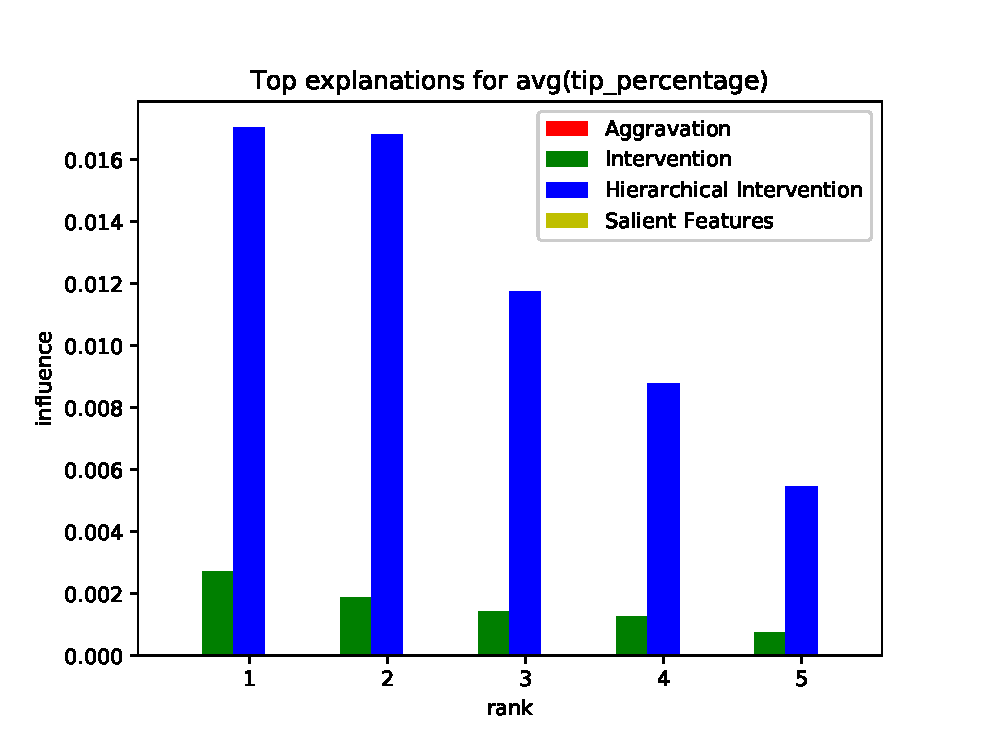
\includegraphics[width=0.96\columnwidth]{images/Top_explanations_for_avg_tip_percentage_influence}
	\caption{Influence for Spatial explanation for average tip percentage(Lower is better)}
	\label{fig:influence_comparison}
\end{figure}

\subsection{K-Folds cross validation}
In order to qualitatively assess the solutions, we use K-Folds cross validation\cite{refaeilzadeh2009cross}. 
%\section{K-Folds Cross Validation}
K Folds cross-validation is a technique for data evaluation\cite{kohavi1995study,refaeilzadeh2009cross}. The data is divided into $k$ parts. One of the parts is used as a training set and the remaining parts are used as test sets. The purpose of the training set is to model the data. Once we have a model, we can use it to classify and/or predict unseen data. The test set is used to evaluate how well the model was trained.

Since we do not have ground truth for our explanations, we have to make a compromise in terms of estimating how good our solution is. Our assumption here is that in general, a good explanation would stand out on unseen data i.e. given a good explanation on part of the data, it would give similar results on unseen parts of the data. This is the same assumption that was made by \cite{chirigati2016data} in their evaluation of the Data Polygamy framework. 
% Add here
We use the first 5 months data from  NYC yellow cab dataset in 2016. The data spanned ~50 million trips. 
%%%%
We split the data into 5 parts. Each month of data forms one part. 
%The data was divides by the month of the year. 
This is because there are specific observable patterns in each month, e.g. weekends have less density of trips than the weekdays for the dataset we evaluated. 
One of the parts is used to find the explanation (the training data). The rest of the data is the test data. 
%We also calculate an explanation of the test data. 
%The relative distance between the explanation index of the test data and the explanation index of the explanation provided by the training data when applied to the test data is used as a measure of evaluation.

%\textbf{Experimental Setup}. We performed the evaluation on the first 5 months of data from the NYC yellow cab dataset from 2016. The data spanned ~ 50 million trips. The $k$ for our evaluation was $5$. This value was chosen after a series of experiments. We wanted the size of each partition to be large enough to support our generalization assumption. If the solution space for evaluation is small, it leads to inconsistent results. Each month represented a partition for a k-folds evaluation. According to our analysis, we found that the approach works very well with low values of alpha. Fig.~\ref{fig:kfolds} shows some of the results of our evaluation for a number of observations. The lower the value of the relative distance, the better the results.

We define the relative distance to measure the quality of the {\explanation}:
%The relative distance in the K Folds cross validation represents how much the explanation impact changes when we look at the explanations in the context of unseen data. A relative distance of zero represents that the explanation has the same impact on unseen data as if we had seen the data. A relative distance of one would represent that the top explanation for the unseen data has nothing in common with the explanation of seen data. Let $e_{test}$ be the explanation index for the test set. Let $e_{train}$ be the explanation index for the training set. Then,
$$relative\_distance = \frac{|e_{test}-e_{train}|}{|e_{test}+e_{train}|}$$
where $e_{train}$ and $e_{test}$ denote the top {\explanation} for the training and test dataset respectively. 
The relative distance metric was chosen because of its nature of showing a steep decline when two solutions do not match. It is also ideal because it caters to the different types of {\fact}s that a user can specify. Since the {\fact} in our system is defined as an arithmetic operation over aggregate queries, they do not have bounds on their values. Thus, it makes relative distance a useful metric for measuring similarity.

\begin{figure}[htp]
            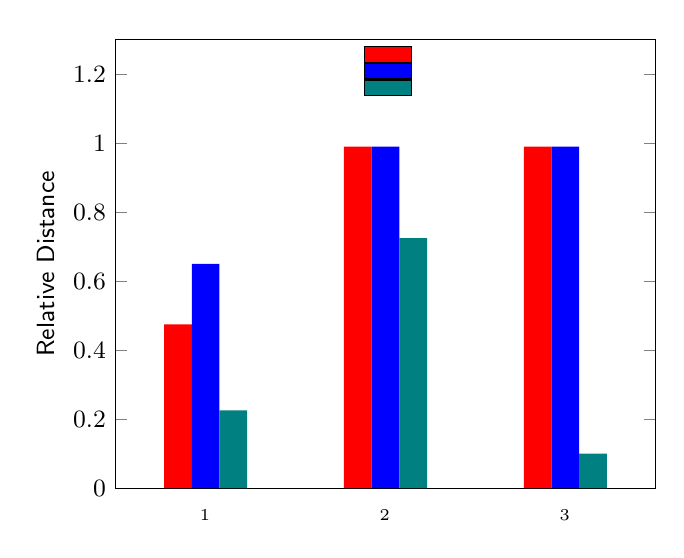
\begin{tikzpicture}
            [every plot/.append style={}]
            \begin{axis}[
                major x tick style = transparent,
                ybar=0*\pgflinewidth,
                bar width=10pt,
%                ymode = log,
%                log origin=infty,
                ylabel = {\small \textsf{Relative Distance}},
                yticklabel style = {font=\small},        
                xticklabel style = {font=\small},
                symbolic x coords={{\fact}$_1$,{\fact}$_2$,{\fact}$_3$},
                xtick=data,
                scaled y ticks = false,
                enlarge x limits=0.25,
                ymin=0,
                ymax=1.3,
                legend cell align=left,
                legend style={
                    column sep=0.6ex,
                    legend columns = 1,
                    draw = none,
                    fill = none,
                    at={(0.6,1)},
                    font=\scriptsize,
                    }
                ]
                        
                \addplot [area legend,draw=none,fill=red]
                coordinates {({\fact}$_1$, 0.475)({\fact}$_2$,0.99) ({\fact}$_3$,0.99) };
                
                \addplot [area legend,draw=none,fill=blue]
                coordinates {({\fact}$_1$,0.65)({\fact}$_2$, 0.99) ({\fact}$_3$,0.99) };
                
                \addplot [area legend,draw=none,fill=teal]
                coordinates {({\fact}$_1$,0.225)({\fact}$_2$, 0.725) ({\fact}$_3$,0.1)};
                
                \legend{\textsf{{\aggravation}}, \textsf{{\intervention}}, \textsf{{\solution}}}
            \end{axis}
        \end{tikzpicture}
    \caption{\small Relative Distance}
    \label{fig:kfolds}
\end{figure}

Here are the {\fact}s that we use in the experiment:
%\newline \newline
%{\bf \textbf{SELECT}}  \textbf{COUNT}(*)  \textbf{AS}  $q_1$  \textbf{FROM} data    
%\newline
%\textbf{WHERE} payment\_type = 1
%\newline \newline
%{\bf \textbf{SELECT}}  \textbf{COUNT}(*)  \textbf{AS}  $q_2$  \textbf{FROM} data    
%\newline
%\textbf{WHERE} payment\_type = 2

\renewcommand{\lstlistingname}{{Fact}}% Listing -> Algorithm
\begin{lstlisting}[language=SQL, caption=q1/q2, label=qry:o1]
Select count(*) as q1 
from data where payment_type=1;

Select count(*) as q2 
from data where payment_type=2;
\end{lstlisting}

\begin{lstlisting}[language=SQL, caption=q1, label=qry:o2]
Select AVG(trip_distance) as q1 
where passenger_count=4;
\end{lstlisting}

\begin{lstlisting}[language=SQL, caption=q1/q2, label=qry:o3]
Select count(*) as q1 
from data where vendorid=1;

Select count(*) as q2 
from data where vendorid=2;
\end{lstlisting}

Figure \ref{fig:kfolds} demonstrates the relative distance of the three {\fact}s mentioned previously. We can observe that both {\aggravation} and {\intervention} have low relative distance, which means that the best {\explanation} in the training data share few common tuples with the best {\explanation} in the test data. Compared to them, the {\explanation} detected by {\solution} have more overlapped tuples in the training data and the test data. 

\subsection{Precision and Recall}
% \begin{wrapfigure}{L}{0.5\textwidth}
%   \begin{center}
%     \includegraphics[width=0.48\textwidth]{outbreakheatmap.png}
%   \end{center}
%   \caption{A heatmap showing sythesized data}
%   \label{fig:synthesized_data}
% \end{wrapfigure}
% \begin{figure}[h]
% \includegraphics[width=\columnwidth]{outbreakheatmap.png}
% \caption{A heatmap showing sythesized data}
% \label{fig:synthesized_data}
% \end{figure}

Since it is very difficult to find datasets with the ground truth we used synthetic datasets to evaluate our solution \cite{maciejewski2009generating}. 
%The synthetic dataset is fabricated using real data from the Indiana Public Health Emergency Surveillance System. This data contains information about Patients in Indiana and their health issues over time and location. 
We can calculate precision and recall using this data \cite{powers2011evaluation}. The data is synthesized in such a way that it shows similar patterns to the actual data. Synthetic data related to outbreaks of certain diseases is synthesized into this data. In order to evaluate our system, we used the temporal component of the outbreak and the type of disease as our {\fact}. To be specific, the synthetic data consisted of an outbreak of Gastrointestinal infection in July. Our observation was the ratio of the number of gastrointestinal infection incidents between June and July when there is an infection against the number of gastrointestinal infection incidents between June and July in synthesized data where there was not an outbreak. Precision and Recall was calculated by comparing the areas of the top ten explanations related to the ground truth with the approximate area covered by the outbreak data. We cannot use the individual points to calculate precision and recall because there is a lot of data unrelated to the outbreak which occurs in proximity. To put things into context, each instance of the synthesized data contains ~2 million records. The data related to the outbreak consists of a few dozen records. 
%Fig.~\ref{fig:synthesized_data} shows a heatmap of all the points in the synthesized data. 
%The outbreak for this particular instance only affects a small part of Indiana to the North West just below Lake Michigan. 
%Fig.~\ref{fig:precisionrecall} shows the points representing the outbreak as well as some of the top polygons returned using Hierarchical Intervention. 
%While our system is designed to work fast on partitioning techniques with no overlaps like K-Means and Greedy Hierarchical Clustering. Some of the clustering approaches that we use which give better results do have overlaps. Thus we used R*-Tree partitioning in our example. The candidate explanations provided by this partitioning techniques can have spatial overlaps.

% \begin{figure}[h]
% \includegraphics[width=\columnwidth]{precisionrecall.png}
% \caption{Synthetic Outbreak data. The circles show the ground truth while the polygons show the relevant explanations produced by our system}
% \label{fig:precisionrecall}
% \end{figure}

Precision can be evaluated by the following equation:
$$Precision = \frac{E \cap O}{E}$$
where $E$ is the area represented by our polygons and $O$ is the area represented by the Outbreak points.

% don't understand the definition (why it is defined like this?)
For calculating recall, we can use the actual outbreak points since it does not require false positives.
$$Recall = \frac{true\_positives}{false\_negatives}$$

\begin{table}[]
	\centering
	\caption{Precision and Recall}
	\begin{tabular}{|c|c|c|c|}
		\hline
		Metric & {\solution} & {\aggravation} & {\intervention} \\ \hline
		Precision & 0.31 & 0.01 & 0.0003\\ \hline
		Recall &  0.74 & 0.04 & 1\\ \hline
	\end{tabular}
	\label{tab:precision_and_recall}
\end{table}


%\subsection{Comparison}
According to the experiment result in Section \ref{sec:spatial_partitioning_methods}, we choose to use R* Tree partitioning method to build the spatial {\explanation}s for its stable and good performance.
Table \ref{tab:precision_and_recall} shows the precision and recall for {\solution}, {\aggravation} and {\intervention}. 
%We compared the precision and recall of Hierarchical Intervention with Aggravation and Intervention.
Our approach {\solution} can achieve 0.31 precision and 0.74 recall respectively. 
%\textbf{Aggravation}. We used the same observation for aggravation that we did for Hierarchical Intervention. From the top ten explanations, only one of the explanation was able to predict one of the 27 correct tuples in the ground truth.
The top 10 {\explanation}s generated by {\aggravation} only can predict one of the 27 correct tuples in the ground truth. Its precision is 0.01 and recall is 0.04.
%$$Precision = 0.01$$
%$$Recall = 0.04$$
%\textbf{Intervention}. Finally, Intervention was used to find an explanation. Since there was only one hospital in the area of the outbreak, Intervention was able to provide that hospital as a relevant predicate in an explanation. This resulted in all the ground truth points being included in the explanation! However, since there are a large number of tuples related to this predicate, it resulted in low precision.
%$$Precision = 0.0003,\ Recall = 1$$
For {\intervention}, its precision and recall are 0.0003 and 1.0 respectively. 
The reason is there was only one hospital in the area of the outbreak. 
Intervention was able to provide that hospital as a relevant predicate in an explanation. 
This resulted in all the ground truth points being included in the explanation! 
However, since there are a large number of tuples related to this predicate, it resulted in low precision.

% \begin{wrapfigure}{r}{0.5\textwidth}
%   \begin{center}
%     \includegraphics[width=0.48\textwidth]{precisionrecall.png}
%   \end{center}
%   \caption{Synthetic Outbreak data. The circles show the ground truth while the polygons show the relevant explanations produced by our system}
% \label{fig:spatial_spatial_vertical}
% \end{wrapfigure}



% \textbf{Influence and Intensity for Hierarchical Intervention}
% \begin{figure}[H]
% 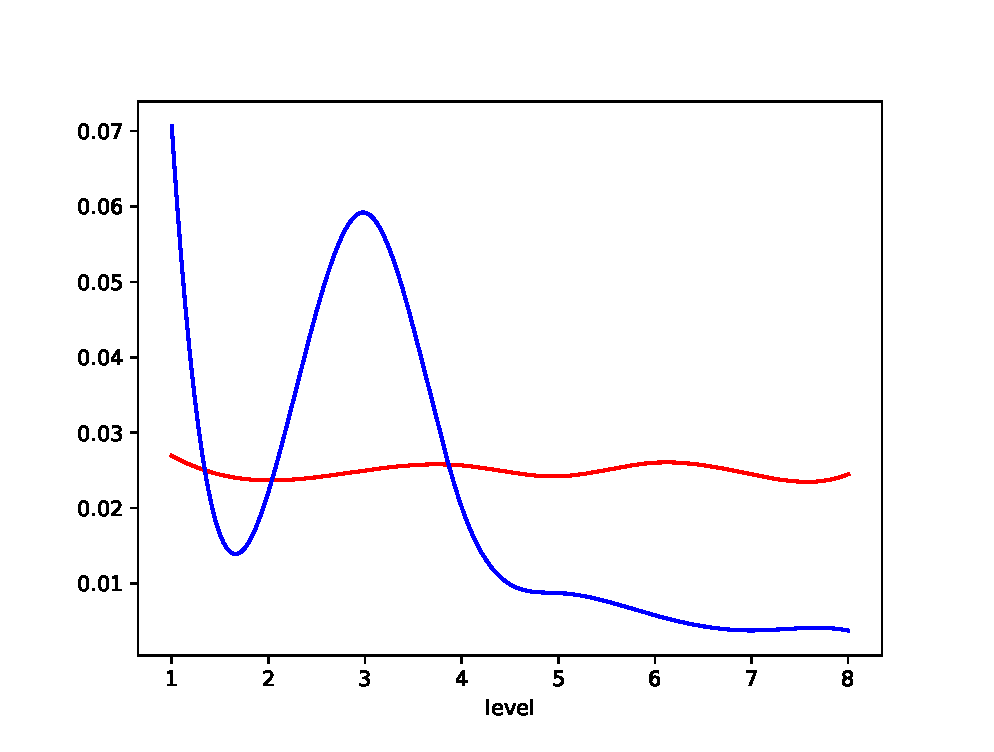
\includegraphics[width=\columnwidth]{heiint_tip_percentage}
% \caption{Comparison of Influence and Intensity against level of hierarchy with average tip percentage as observation}
% \label{fig:hieint_tip_percentage}
% \end{figure}




% \begin{figure}[H]
% 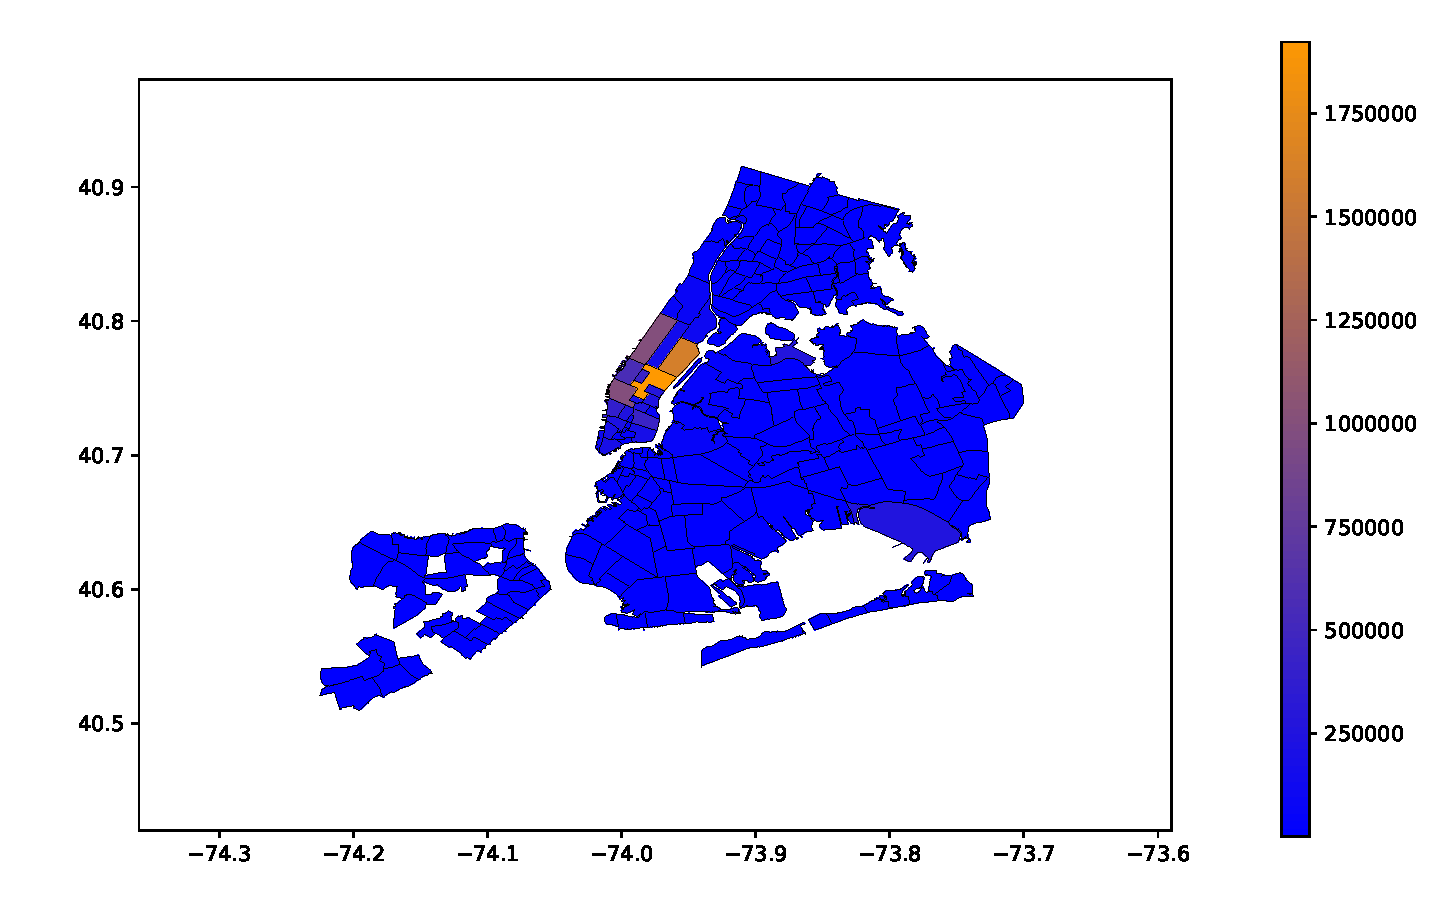
\includegraphics[width=\columnwidth]{count_initial}
% \caption{The number of trips for each zone by pickup zone}
% \label{fig:count_initial}
% \end{figure}

% \begin{figure}[H]
% 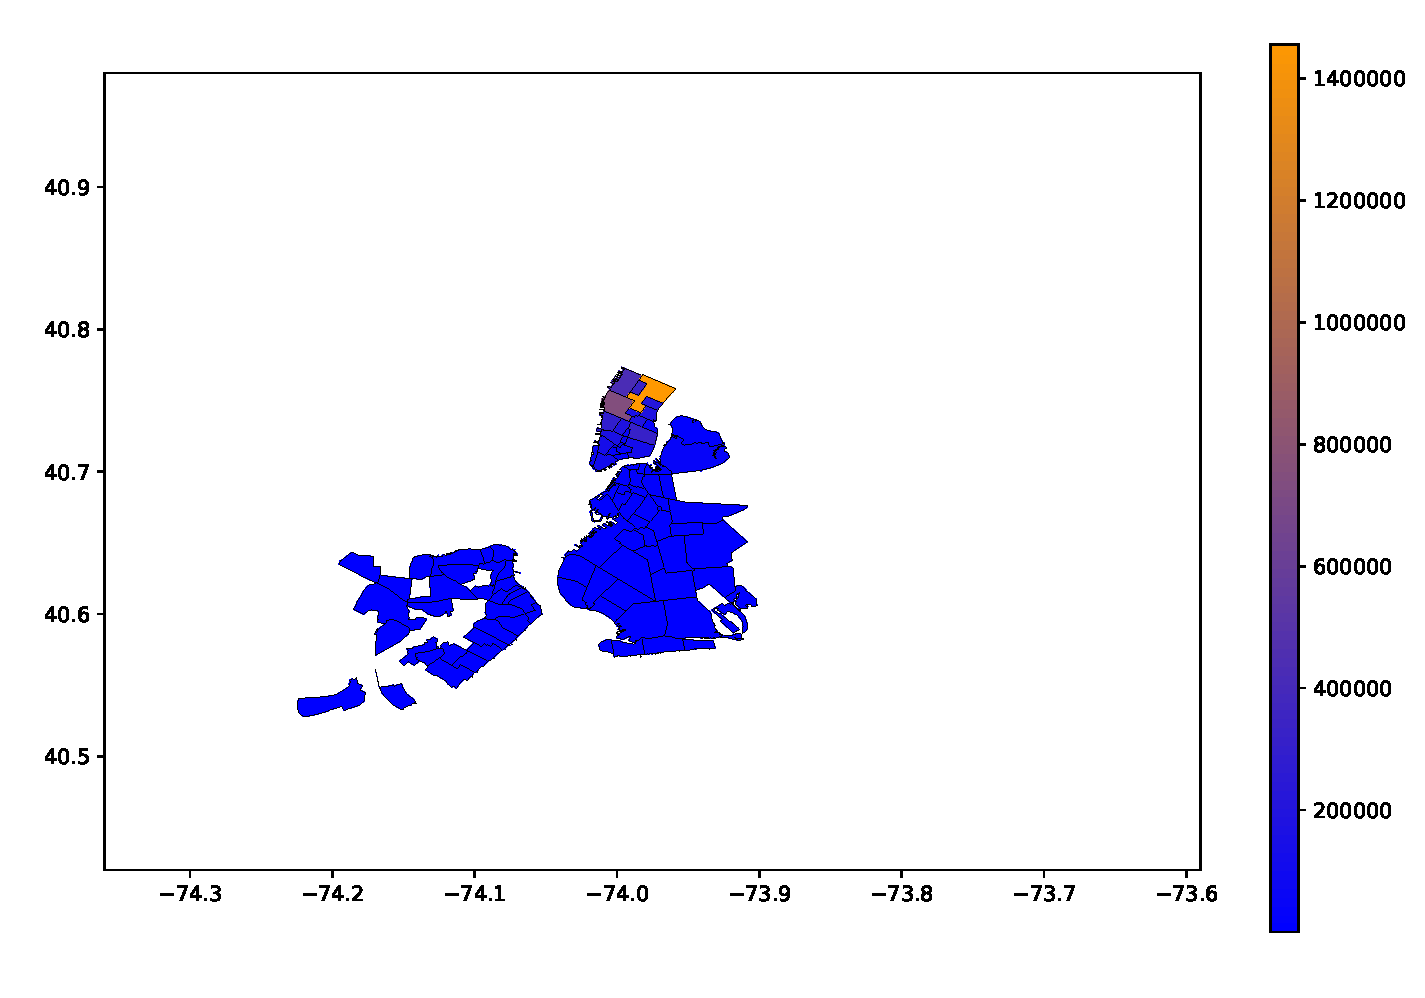
\includegraphics[width=\columnwidth]{top_level_2}
% \caption{Number of rows that represent the top explanation for average tip percentage at level 2}
% \label{fig:top_level_2}
% \end{figure}

% \begin{figure}[H]
% 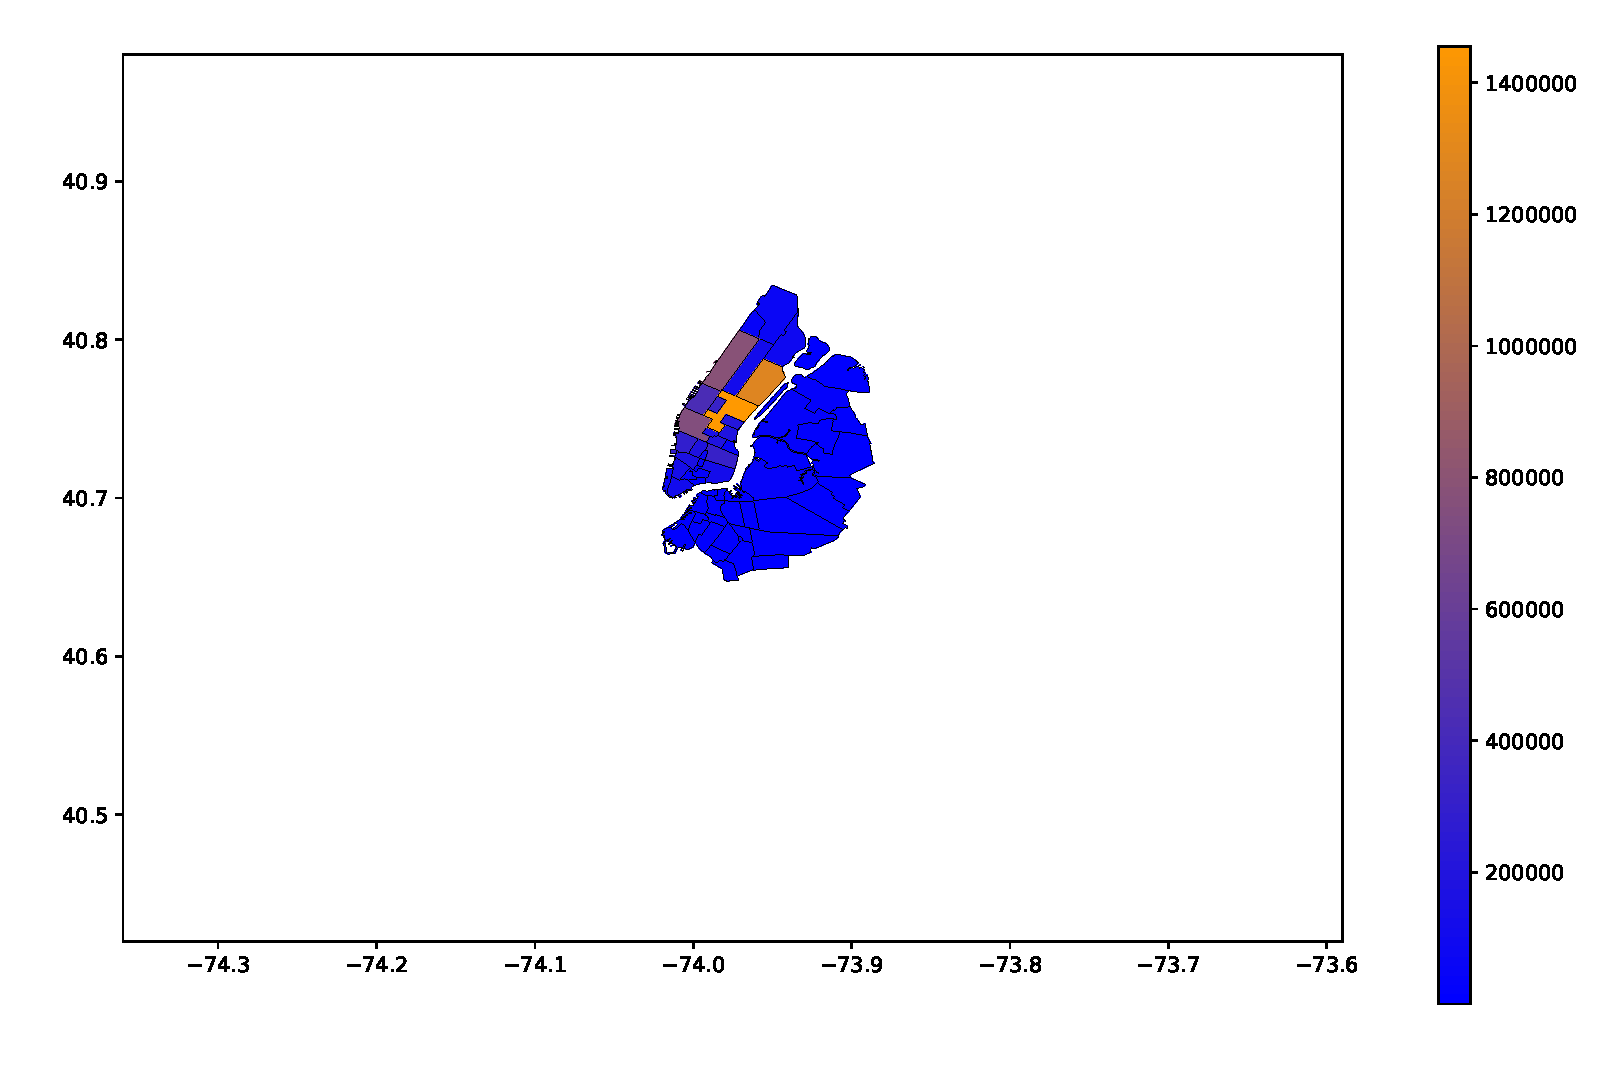
\includegraphics[width=\columnwidth]{top_level_3}
% \caption{Number of rows that represent the top explanation for average tip percentage at level 3}
% \label{fig:top_level_3}
% \end{figure}

% \begin{figure}[H]
% 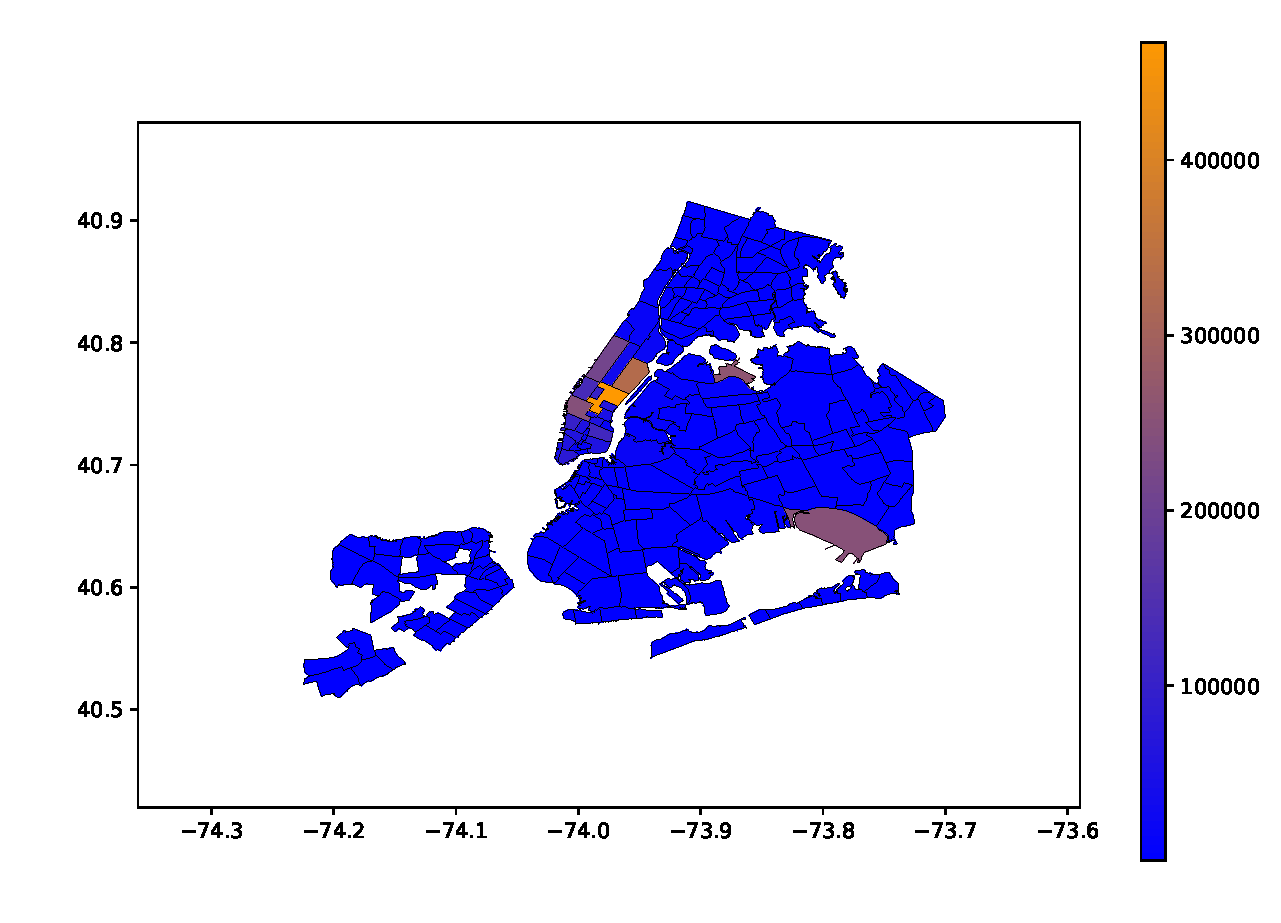
\includegraphics[width=\columnwidth]{level_3_removed}
% \caption{The cartogram for the data when we remove he level 3 explanation}
% \label{fig:level_3_removed}
% \end{figure}


\subsection{Speed and Scalability}
\label{sec:speed}
The speed of each approach is simply the time taken to calculate the explanations. The time varies depending on the size of the data. For performance evaluation, we used the NYC TLC data for 2016. The data is divided into months. As we increase the number of months to be processed, the time taken for each approach increases almost linearly for aggravation, intervention and hierarchical intervention. For salient features, the time increases slightly exponentially. The results of our evaluation are displayed in Fig.~\ref{fig:performance}

%\textbf{Experimental Setup}. The speed of each approach is simply the time taken to calculate the explanations. Since all the approaches are implemented on top of distributed systems, the time varies depending on the number of nodes used. We experimented with calculating explanations for 1,3, and 5 months in a distributed environment. For the cluster, we used Google Compute Engine nodes(1 vCPU, 3.5GB RAM, 4 nodes). All the nodes in our cluster had the same specifications. The Aggravation, Intervention and Hierarchical Intervention were tested on Apache Spark running on YARN while the Salient Features were generated with the Data Polygamy Framework running on YARN.
\begin{figure}[h]
	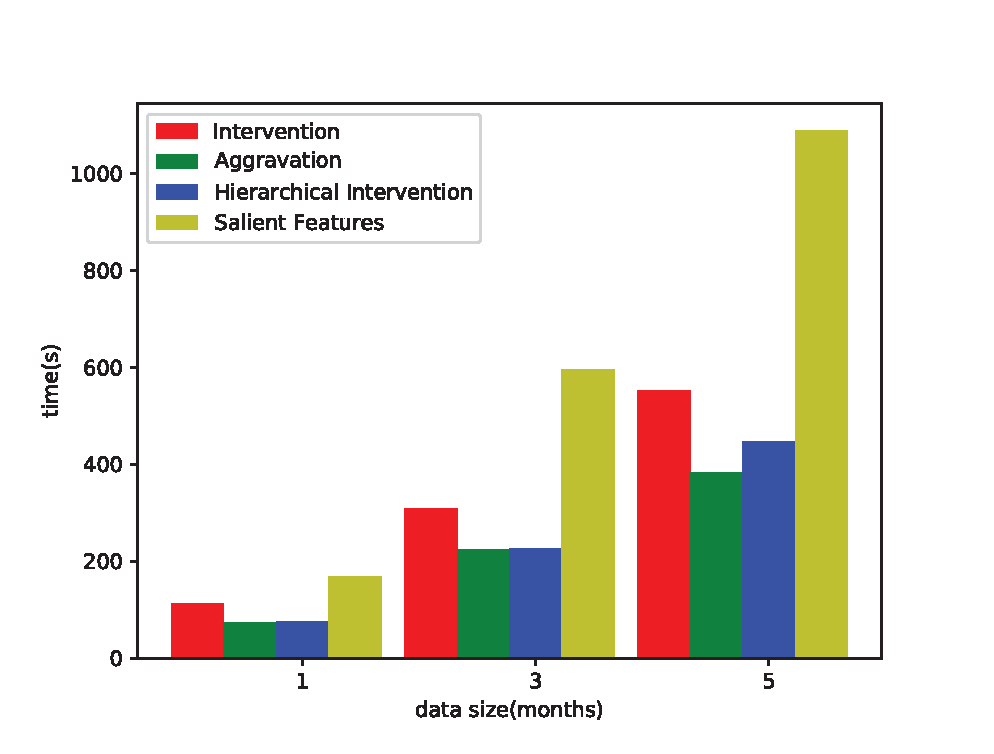
\includegraphics[width=\columnwidth]{images/performance.eps}
	\caption{Time taken by each approach as we increase the size of data}
	\label{fig:performance}
\end{figure}
The run times that were observed can be explained as follows. Aggravation takes the least amount of time of the compared approaches. Intervention costs more than aggravation because it includes the additional step of calculating statistics for the attributes as well as iterating the table. Hierarchical Intervention takes more time than aggravation but less time than intervention. This is because of several factors. One of the factors is that when we are using intervention and aggravation, we are using several attributes, on the other hand, hierarchical intervention only uses the spatial attribute. On the other hand, we are creating a hierarchy. The in the case of this analysis we only used one query as the observation for the sake of comparison. However, multiple queries can affect the comparison as well. The time taken by Salient Features is also affected by a number of factors. First, the implementation of the salient features that we use is the one used in the Data Polygamy Framework \cite{chirigati2016data}. This approach uses the MapReduce framework. The other approaches use the Spark framework. Since Spark makes use of an execution plan which is more efficient than MapReduce, it is a factor in the slower runtime of the Salient Features approach. Thus, when comparing salient features to the other approaches, this can be considered something similar to black box testing. The most expensive computation step in salient features is the interpolation step which does not occur in the other approaches.


% \begin{figure}[H]
% 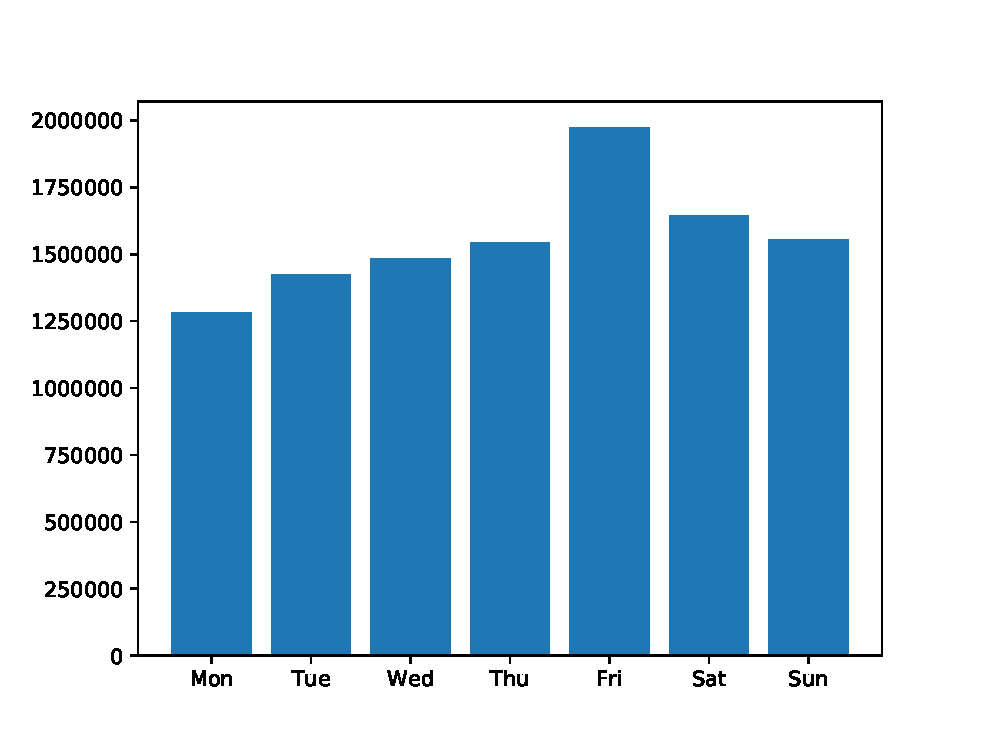
\includegraphics[width=\columnwidth]{day_comparison}
% \caption{Number of trips against trip day}
% \label{fig:day_comparison}
% \end{figure}
